\documentclass{sigchi}

% Use this section to set the ACM copyright statement (e.g. for
% preprints).  Consult the conference website for the camera-ready
% copyright statement.

% Copyright
%\CopyrightYear{2017}
%\setcopyright{acmcopyright}
%\setcopyright{acmlicensed}
%\setcopyright{rightsretained}
%\setcopyright{usgov}
%\setcopyright{usgovmixed}
%\setcopyright{cagov}
%\setcopyright{cagovmixed}
% DOI
%\doi{http://dx.doi.org/10.475/123_4}
% ISBN
%\isbn{123-4567-24-567/08/06}
%Conference
%\conferenceinfo{CHI'16,}{May 07--12, 2016, San Jose, CA, USA}
%Price
%\acmPrice{\$15.00}

% Use this command to override the default ACM copyright statement
% (e.g. for preprints).  Consult the conference website for the
% camera-ready copyright statement.

%% HOW TO OVERRIDE THE DEFAULT COPYRIGHT STRIP --
%% Please note you need to make sure the copy for your specific
%% license is used here!
% \toappear{
% Permission to make digital or hard copies of all or part of this work
% for personal or classroom use is granted without fee provided that
% copies are not made or distributed for profit or commercial advantage
% and that copies bear this notice and the full citation on the first
% page. Copyrights for components of this work owned by others than ACM
% must be honored. Abstracting with credit is permitted. To copy
% otherwise, or republish, to post on servers or to redistribute to
% lists, requires prior specific permission and/or a fee. Request
% permissions from \href{mailto:Permissions@acm.org}{Permissions@acm.org}. \\
% \emph{CHI '16},  May 07--12, 2016, San Jose, CA, USA \\
% ACM xxx-x-xxxx-xxxx-x/xx/xx\ldots \$15.00 \\
% DOI: \url{http://dx.doi.org/xx.xxxx/xxxxxxx.xxxxxxx}
% }

% Arabic page numbers for submission.  Remove this line to eliminate
% page numbers for the camera ready copy
% \pagenumbering{arabic}

% Load basic packages
\usepackage{balance}       % to better equalize the last page
\usepackage{graphics}      % for EPS, load graphicx instead 
\usepackage[T1]{fontenc}   % for umlauts and other diaeresis
\usepackage{txfonts}
\usepackage{mathptmx}
\usepackage[pdflang={en-US},pdftex]{hyperref}
\usepackage{color}
\usepackage{booktabs}
\usepackage{textcomp}

% Some optional stuff you might like/need.
\usepackage{microtype}        % Improved Tracking and Kerning
% \usepackage[all]{hypcap}    % Fixes bug in hyperref caption linking
\usepackage{ccicons}          % Cite your images correctly!
% \usepackage[utf8]{inputenc} % for a UTF8 editor only

% If you want to use todo notes, marginpars etc. during creation of
% your draft document, you have to enable the "chi_draft" option for
% the document class. To do this, change the very first line to:
% "\documentclass[chi_draft]{sigchi}". You can then place todo notes
% by using the "\todo{...}"  command. Make sure to disable the draft
% option again before submitting your final document.
\usepackage{todonotes}

% Paper metadata (use plain text, for PDF inclusion and later
% re-using, if desired).  Use \emtpyauthor when submitting for review
% so you remain anonymous.
\def\plaintitle{SHECC: A Smart Home Energy Cruise Control}
\def\plainauthor{Francesco Fraternali, Sean Hamilton}
\def\emptyauthor{}
\def\plainkeywords{Smart Home; Energy; Environment; Budget; Money; Instant Feedback}
\def\plaingeneralterms{Documentation, Standardization}

% llt: Define a global style for URLs, rather that the default one
\makeatletter
\def\url@leostyle{%
  \@ifundefined{selectfont}{
    \def\UrlFont{\sf}
  }{
    \def\UrlFont{\small\bf\ttfamily}
  }}
\makeatother
\urlstyle{leo}

% To make various LaTeX processors do the right thing with page size.
\def\pprw{8.5in}
\def\pprh{11in}
\special{papersize=\pprw,\pprh}
\setlength{\paperwidth}{\pprw}
\setlength{\paperheight}{\pprh}
\setlength{\pdfpagewidth}{\pprw}
\setlength{\pdfpageheight}{\pprh}

% Make sure hyperref comes last of your loaded packages, to give it a
% fighting chance of not being over-written, since its job is to
% redefine many LaTeX commands.
\definecolor{linkColor}{RGB}{6,125,233}
\hypersetup{%
  pdftitle={\plaintitle},
% Use \plainauthor for final version.
%  pdfauthor={\plainauthor},
  pdfauthor={\emptyauthor},
  pdfkeywords={\plainkeywords},
  pdfdisplaydoctitle=true, % For Accessibility
  bookmarksnumbered,
  pdfstartview={FitH},
  colorlinks,
  citecolor=black,
  filecolor=black,
  linkcolor=black,
  urlcolor=linkColor,
  breaklinks=true,
  hypertexnames=false
}

% create a shortcut to typeset table headings
% \newcommand\tabhead[1]{\small\textbf{#1}}

% End of preamble. Here it comes the document.
\begin{document}

\title{\plaintitle}

\numberofauthors{2}
\author{%
  \alignauthor{Francesco Fraternali\\
    \affaddr{University of California, San Diego}\\
    \email{e-mail address}}\\
  \alignauthor{Sean Hamilton\\
    \affaddr{University of California, San Diego}\\
    \email{skhamilt@eng.ucsd.edu}}\\
}

\maketitle

\begin{abstract}
  We did some shit for a class
\end{abstract}

\category{H.5.m.}{Information Interfaces and Presentation
  (e.g. HCI)}{Miscellaneous} \category{J.7}{Computers in Other Systems}{Consumer products}

\keywords{\plainkeywords}

\section{Introduction}

Will data fusion dashboards for smart homes allow their owners to make better decisions for reducing total home energy consumption?

We hypothesize that, if smart home energy consumption data is aggregated, correlated, and displayed in an easy to digest manner on dashboard, the user will be more conscience of which "knobs" should be adjusted to reduce energy consumption and which will only reduce comfort, or more generally Quality of Experience (QoE), while not providing substantial enough savings.

This paper will contribute to the fields of Human-Computer Interaction (HCI) and Internet of Things (IoT). How useful the fusion of smart home data is to its user will be explored. In addition various ways of presenting energy usage information will also be examined and how presentation of the data affects the users decisions in reducing the energy consumption for the home.

\section{Related Work}

Some smart homes provide a lot of data about energy consumption of various devices and the entire home [1,3], but we believe that today's interfaces to the systems do not enable a person to know which settings matter with respect to reducing energy consumption. As result the users often make uninformed decisions to cut energy usage as it is very difficult to figure out what really matters, e.g. should I turn up my refrigerator, twiddle with my HVAC system, dim my lights or replace with lower wattage bulbs, or turn down my water heater. People mostly rely on manual settings that are not changing overtime even if external condition may change (e.g. seasons). Similar work has been done that uses machine learning algorithms to solve the problem of reducing energy consumption while maintaining an acceptable QoE [1,2,4]. These algorithms however cannot account for the various subjective human factors that may affect the decisions of what controls to adjust that don?t sacrifice comfort, e.g. a sick person may like a slightly warmer home or in the summer the A/C is used to reduce humidity for comfort as well a temperature.

\section{Method}

\subsection{Design}

We will use a simulation of a home running various energy scenarios that the participants will interact with. The simulation will have similar controls to those found in the homes today such as 1 -10 setting for the refrigerator, temperature set points for HVAC, and lighting controls. The simulation will provide how much energy is used and a comfort level, or Quality of Experience (QoE) measured 1 - 10, for a scenario based on the settings of the controls. The values used for energy usage will be obtained from manufacture specifications and studies on energy consumption averages of various systems. The QoE calculation will be a simplified model based on the work presented in [2].

A control group of participants will be asked to change the various controls as they think they should to save energy in the various scenarios in the same way they would in there own homes. The experimental group of participants will be given access to the same controls and scenarios as the control group but with the addition of a smart dashboard which displays hot spots of energy consumption and historical energy usage to aid in making the decision of which controls to change and to what settings.

We will measure the energy used by considering typical power consumptions for each device selected and for each environment (e.g. HVAC for a Small Home needs to consume less power to air conditioning compared to an HVAC used for a Large Home, while the refrigerator would probably use the same power to operate). Hence, we will multiply the average power consumption values with the set up of each participant and calculate then the total energy consuming. The result could look like Fig 1.

\subsection{Evaluation}

If the use of a fusion dashboard leads to users making decisions that substantially reduce energy consumption while maintaining a reasonable QoE compared to people that do not use it then are hypothesis is supported. Otherwise we can cannot conclude that a smart dashboard is ineffective because our sample size may be insufficient or other variables not accounted for may be in play and a further analysis of the problem would need to be conducted.

\section{Results}

\begin{figure}
\centering
  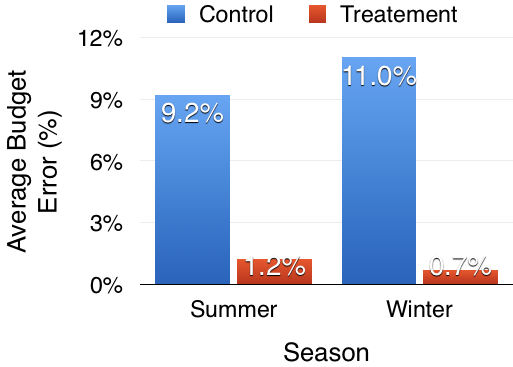
\includegraphics[width=0.9\columnwidth]{figures/errors}
  \caption{Percentage of budget error by season for control and treatment groups }~\label{fig:figure1}
\end{figure}

\begin{figure}
\centering
  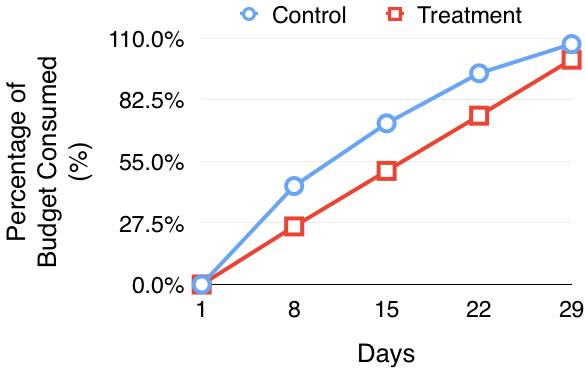
\includegraphics[width=0.9\columnwidth]{figures/budget}
  \caption{Percentage of budget consumed over time for control and treatment groups}~\label{fig:figure2}
\end{figure}

\begin{figure}
\centering
  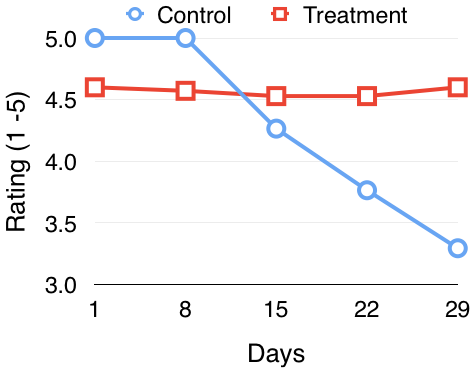
\includegraphics[width=0.9\columnwidth]{figures/comfort}
  \caption{Comfort levels over time for control and treatment groups}~\label{fig:figure3}
\end{figure}

\section{Discussion}

\section{Conclusion}

% BALANCE COLUMNS
\balance{}

% REFERENCES FORMAT
% References must be the same font size as other body text.
\bibliographystyle{SIGCHI-Reference-Format}
\bibliography{main}

\end{document}

%%% Local Variables:
%%% mode: latex
%%% TeX-master: t
%%% End: